\chapter{Problem Analysis}

In the introduction section of this thesis, we defined a list of design elements \textbf{E1}~--~\textbf{E6} that we are going to
implement in our game. We have also presented the notion of modifiability and examined some of
the numerous Minecraft mods to see which parts of a game can be modified. In this section, we are
going to look at the different tools, libraries and engine design possibilities that could potentially
be used to implement our game.

\section{Modding Tools}

In the first chapter, we investigated different possible ways in which we can make our game modifiable and defined a list of aspects
we would like to allow our players to change. In this section we examine different tools we can create and provide to our players
for mod creation. These tools should satisfy our goals, that is they should allow our players to create and modify
entities \textbf{(G2.1)}, alter the game progression \textbf{(G2.2)} and should also produce mods that are easily installable
by other players \textbf{(G3)}.

Modding tools can generally be of two types:
\begin{itemize}
    \item An API that can be used in a scripting language.
    \item An editor, good examples being world editors in the Warcraft~3~\cite{WC3} and
        Starcraft~\cite{SC} games.
\end{itemize}

\subsubsection{API}

This option would require us to create an interface in which functionality of the engine binds to functions that can be called
from a scripting language embedded within the engine. This would allow our players to write scripts that can be loaded at the
start of our game or during its runtime and can change anything provided by the interface.

An example of such API can be found in the game Starbound~\cite{Starbound}, which allows its
players to create modifications by using its Lua API to write scripts. An example of a simple Starbound script,
which defines a new object in the game that spawns a chicken when the player interacts with it,
can be seen in Figure~\ref{sb-lua-mod-ex}. Here, the mod creator defined two functions called \emph{init} and
\emph{onInteraction}. These two functions are defined by the game and are called by it
-- \emph{init} is called when the object is place into the world and \emph{onInteraction} is called
whenever the player interacts with the object. The game also provides each mod with several tables that
help the mod to interact with the game world -- in this case the mod uses the \emph{object} table, which
represents each instance of the spawner object, and \emph{world}, which represents the game world and
is shared between all objects.

\begin{figure}[h]
    \centering
    \begin{lstlisting}
function init()
    object.setInteractive(true)
end

function onInteraction()
    world.spawnMonster("chicken",
                       {0, 0}, {level = 10})
end
    \end{lstlisting}
    \caption{A simple script that represents an interactive monster spawner. When the player interacts
            with this object it spawns a level 10 chicken at the absolute coordinates (0, 0).}
    \label{sb-lua-mod-ex}
\end{figure}

This option allows us to provide a large amount of our engine's functionality and data wrapped in an easy to use interface, which can lead
to the ability to easily modify it and thus satisfying our goal \textbf{(G2.1)}. This interface can also contain functions that handle the
game's wave system and allows the mod creators to modify wave composition and delays between waves, which would satisfy our goal
\textbf{(G2.2)}. To satisfy the last of the three goals, \textbf{(G3)}, we can design the scripting system of our game in a way that only
requires the players to place a downloaded script in a directory and register the script in a config file.

Besides making the game modifiable, this approach can lead to faster development~\cite{GEA} since parts of the game that are not performance
critical can be written in an interpreted language. This would avoid long recompilation times that
may be needed when we would change a piece of the code base written in a language that needs to be compiled and also allow 
us to prototype new features and bug fixes
without the need to restart the game as many of these interpreted language can execute pieces of code passed to them as strings.
Additionally, using a higher level language would make the mod creation process easier for non-programmers~\cite{WhyScripting}.

Because of the ease of implementation, satisfaction of our goals, the above mentioned side benefits this option has on the
development of the game and the fact that it provides more control for the mod creators -- as explained in the following subsection --
we decided to choose it for our game.

\subsubsection{Editor}

A game editor is an external window application used to modify a game. In most cases it's used to edit maps or scenarios for the game.
But since the maps in our game are created by the player -- by destroying walls and creating buildings -- we are more interested in a
different aspect of editors and that is changing entities in the game. In Figure~\ref{sc-editor} we can see an example of such editor.
It allows its user to select an entity and change its attributes, such as health, placing cost, type, model and the user can even 
select which predefined abilities and behavior the entity uses. An editor could easilly be used to define the composition of enemy
waves and the delays between waves, satisfying our goal \textbf{(G2.2)} and would allow easy mod installation -- as required by our goal
\textbf{(G3)} -- by producing files that can be placed in the game's directory.

\begin{figure}[h]
    \centering
    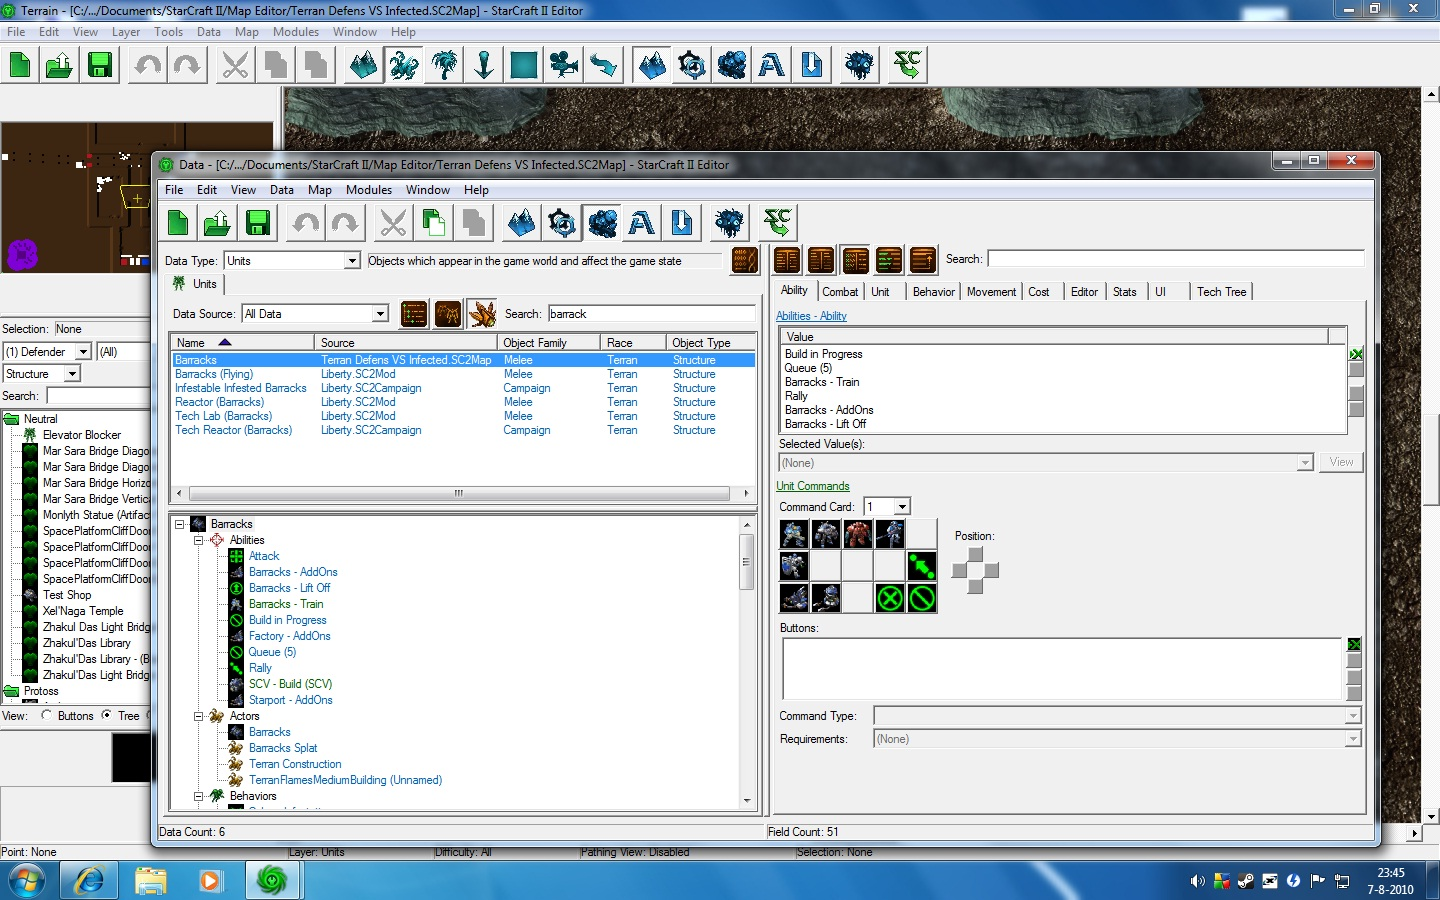
\includegraphics[width=10cm]{../img/sc_editor.jpg}
    \caption{Besides map editing, some editors -- like the Starcraft editor in this figure -- can be used to edit entities.
             \\Source: \href{http://www.darvo.org/images/Tutorials\%20Starcraft\%202/Adding\%20Units\%20to\%20a\%20Building\%20part\%201.jpg}
             {http://www.darvo.org}}
    \label{sc-editor}
\end{figure}

While this approach could be easily implemented using configuration files for entities, our goal \textbf{(G2.1)} requires the ability
to alter the behavior of entities which includes creating entirely new behavior and thus only selecting predefined AI won't suffice.
To achieve this, we could require our users to write the behavior using a scripting language, which wouldn't be much different
from the previous option. Alternatively, we could create a graphical tool that would allow the user construct the behavior out of blocks
representing decisions and actions which would then be translated to source code -- again, requiring a scripting language interfaced
to the engine. An example of such graphical tool is the blueprint system used by Unreal Engine~\cite{UE}.

\begin{figure}[h]
    \centering
    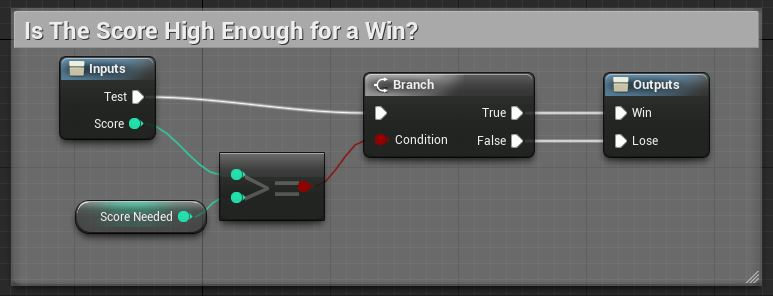
\includegraphics[width=10cm]{../img/blueprints.jpg}
    \caption{A simple blueprint checks if a person passes a test.
             \\Source: \href{://docs.unrealengine.com/latest/images/Engine/Blueprints/UserGuide/Macros/score\_comparison\_example\_macro.jpg}
             {http://www.unrealengine.com}}
    \label{ue-blueprints}
\end{figure}

In Figure~\ref{ue-blueprints} we can see an example blueprint created in Unreal Engine, it comprises interconnected blocks that represent
conditions, loops, actions and other constructs that can be found in a typical programming language. The user uses these blocks to
create programs in a more user friendly manner. Unreal Engine then uses these blueprints to generate C++ code that is then used in the game.

Since we want the mods for our game to be easy to create, implementing an editor would be ideal as it would open modding to an even
broader audience. But implementing a system that is similar to Unreal Engine's blueprints would be far out of the scope of this thesis,
though it might be a good future addition to the project.

\section{Programming Language}

The first tool we need to decide on is the programming language we are going to write our game in.
This choice affects multiple aspects of the final game. These aspects can include, but are not limited to:

\begin{itemize}
    \item Performance: Interpreted languages tend to be slower than compiled languages, but this
        does not to be always true due to the existence of Just-In-Time -- often abbreviated as \emph{JIT} -- compilers, 
        which can provide compilation
        to machine language at program start and runtime optimizations to increase the performance.
    \item Speed of development: Lower level languages often require the implementation of tools that
        are provided by the standard libraries of higher level languages.
    \item Modifiability: Some programming languages -- e.g. interpreted ones -- provide means to
        alter the source code at runtime, while other require recompilation or the use of an embedded language.
\end{itemize}

The programming language that will be used to create our game needs to have one or more libraries that will allow us
to create 3D graphics and be fast enough to offer at least the minimum acceptable framerate while rendering game objects
to the screen, updating the state of the game and processing user input. It should also allow our players to modify the game
even if they only have the distributed version of the game -- meaning it should be able to load code it was not originally compiled
with.

Since mod development requires testing of the mod's functionality in the game, it would be beneficial if the game allowed
our mod creators to change the game's mechanics and data at runtime so that they do not need to restart the game
to see what effect does a change in their mod have on the game. This means that the ability to execute a piece of code
input as a string or load source files during runtime is a feature our programming language should provide.
Lastly, the language should allow us to create a modding API that can be provided to our users as discussed in the previous section.

Aside from these important characteristics, the language should also be easy to use by those of our players that decide to
modify the game.

\subsection{Native Language: C++}

C++, the first language we are going to look at and also the language we ended up choosing, was for a long time the
industry standard when it comes to video games. One of the main reasons for this was that it is -- unlike some of its
rivals, e.g. C\# or Java -- a language that is native, i.e. compiles directly into machine code of a specific processor, 
which generally results into faster executed code.

This benefit of the language, while still present, got weakened by the rise of JIT compilers as both C\# and Java can now
compile their intermediate language the first time it's executed. Since by the time this compilation takes place the
compiler knows what operating system, architecture and hardware specification it compiles for it can provide optimization that
a C++ compiler cannot perform, achieving comparable execution speeds.

Even though the performance gap between these languages got reduced, the era of C++ being one of the most used programming languages
in game development has resulted into an abundance of game programming related materials like libraries, tutorials and books.

One of our main requirements for a programming language is the ability to load code it was not originally compiled with. C++ allows this
with the use of dynamically loaded libraries, but this approach is not easy to use by our mod creators as they would be required to
directly interface their mods with the C++ code of the game's engine. An alternative to this approach is to use more user friendly
language embedded into C++ -- e.g. Lua -- and handle the interface between C++ and this language ourselves. This option also
allows the execution of a code input to the game at runtime, which satisfies another of our requirements.

The reason we decided to choose C++ as the language our game is going to be written in is mainly a combination of the abundance of
various game development related resources aimed at C++ -- be it books, tutorials or even answered questions that can be found
on internet -- and the author's knowledge of the language.

\subsection{Managed Languages: Java and C\#}

Managed languages, unlike native ones such as C++, are compiled to an intermediate language which can then either
be interpreted by a virtual machine or JIT compiled into machine code of the target architecture. The use
of a JIT compiler allows execution speeds that are comparable to those of C++.

Where they beat C++ is in their approachability, as they abstract memory management and other lower level aspects of programming
from the programmer. As such, use of these languages would lead to an easier mod making process for our players, but as
we have already settled in the previous section, that can be done in C++ using an embedded language with easier to
understand syntax and semantics.

Both of the managed languages that were taken into consideration -- Java and C\# -- provide an easy way to execute code input
at runtime using either the Java Compiler API~\cite{JavaCompAPI} or the Roslyn sompiler service~\cite{Roslyn} available in C\#.
Alongside this feature both languages offer the ability to embedd another language throu the use of libraries such as
LuaJ~\cite{LuaJ} or NLua~\cite{NLua}.

The difference of these two languages lies in their environment. The Java Virtual Machine -- often abbreviated as JVM -- provides
the ability to compile the code once and then run the resulting executable file anywhere, which can be beneficial for an ordinary
desktop application. When it comes to games, this advantage loses part of its strength due to the fact that the majority of the
players use a Windows operating system -- as can be seen in the Steam hardware and software survey~\cite{SteamHW}. According
to the survey, over 95\% of the players that use the Steam platform  play their video games on a Windows system -- ranging
from Windows XP to Windows 10. In this case, the use of a virtual machine -- be it JVM or .NET's Common Language Runtime -- brings
little to no advantage over a native language such as C++ in terms of portability. On the other hand, Java gains a disadvantage
compared to C\# as it requires the player to have the JVM installed, which is not installed on any of these operating systems
by default. This means that our game would require the installation of a third party software -- though the JVM can be bundled
with the distributed game, it would still ask our players to install updates. The necessity of having the .NET platform
installed is not a problem as it is developed by Microsoft,
which is also the developer of the Windows operating systems, and as such can be installed through Windows and automatically kept
up to date by the Windows Update service.

Because of this problem, the Java programming language was not chosen for the implementation of our game. C\#, on the other hand,
is an easier to use language than C++ and offers the ability to be modded in itself. Being able to have our game to be modded
in C\# would be beneficial seeing as the Unity3D game engine~\cite{Unity} uses it for scripting and thus many game developers
and modders are already capable of using it. Considering these characteristics of the language, we find it to be equal -- if not
superior -- to C++ in terms of game development capability. The reason for not choosing C\# as the language to write our game in
was the fact that the author has more experience with C++.

\section{Scripting Language}

Now that we have chosen C++ as the programming language we are going to implement the engine of our game with, we need
to choose which language we are provide our modding interface in. Such a language should be easily embeddable within C++,
easy to use and well known in the modding community so that people with modding experience can easily create mods for our game.

\subsection{Lua}

Lua is a programming language that was designed to be embedded into other languages like C or C++ and as such
provides a simple to use API written in ANSI C allowing easy function
binding and data sharing between C/C++ and Lua. These characteristics, along with others such as small memory
footprint, easy to understand syntax and
high configurability using provided meta mechanisms, caused Lua to become the most favorite language used for game 
scripting~\cite{EngineSurvey}.

Due to the high amount of games using Lua for scripting -- e.g. the Wikipedia category called "Lua scripted video games" contains
157 entries~\cite{LuaScriptedVGs} -- there is already a large amount of mod creators that know how to use the language to
create mods for games and as such the use of Lua in our game would make our modding tools more familiar to players that already have
experience in modding.

The ability to easily embedd Lua to our engine written in C++ along with the familiarity the modding community already has with the
language were the main reasons for choosing Lua as the scripting language for our game.

\subsection{Python}

While Python is similar to Lua with its easy to understand syntax, its ability to be embedded to C++ is bit worse in comparison.
The various C++/Python interface APIs are mostly designed to allow the extension of Python using C++ and as such require more
work to embedd Python in C++ -- e.g. unlike Lua, which uses a special stack to communicate with C++, the CPython API~\cite{CPython}
requires manual reference decrementing and incrementing for heap allocated Python objects used in C++.

Where Python generally beats Lua is the abundance of libraries it has available, ranging from scientific libraries to image manipulation
libraries. But since our scripting language will be mainly be used as an interface to the functionality of our engine, these libraries
offer little to no advantage over Lua's minimalistic standard library.

The main downside of using Python as our scripting language is in the fact that Lua is used more often as a scripting language in games
-- the Wikipedia category called "Python scripted video games" contains 17 entries~\cite{PythonScriptedVGs}, which is much lower
than Lua's 157 entries. This means that the modding community will probably not be used to writing mods in Python as much as they are
in Lua. This downside, along with the significant whitespace Python uses -- which might be a bit confusing to a non-programmer that
would want to mod our game -- were the main reasons for choosing Lua over Python.

\subsection{AngelScript}

AngelScript~\cite{AngelScript}, similarly to Lua, is a programming language designed to be embedded into other languages for scripting.
The main advantage it has over Lua is that it is even easier to embedd within C++ because of its C++-like design, requiring only
a simple registration of C++ functions in order to be able to call them.

This advantage is also the main downside of the language, as its C++-like syntax is not as easy to understand as Lua's. This means that while
AngelScript would be easier to embedd into the engine, the modding API wouldn't be as begginer friendly as if it were interfaced
to Lua. Because of this downside and a smaller amount of games that use -- according to the official website~\cite{AngelScriptGames}, 
only 35 games use AngelScript for scripting -- we have decided to choose Lua over AngelScript.

\section{Entity Representation}

In this section, we are going to investigate different approaches for entity representation in our engine, that is, how is each
entity -- i.e. anything that is part of the game world, such as a minion, a wall, a trigger, a task or an event -- will be
structurally represented in our engine. This includes the entity's data, logic and relationships between different entities.

Since our goals \textbf{(G2)}, \textbf{(G2.1)} and \textbf{(G1.1)}, our requirements for the entity representation are:
\begin{itemize}
    \item Extensibility: It should allow easy addition of new entity types so that mods can define new entities for their mods. It
        should, if possible, also allow this extensibility at runtime, which would provide means for easy runtime testing and prototyping.
    \item Modifiability: It should allow easy modification of predefined entity types so that mods can change entities that are already
        present in the unmodded game.
    \item Ease of Lua binding: It should be easily representable in Lua scripts.
    \item Performance: Since the entity updating will, along with rendering, take the majority of execution time, the representation should
        allow fast entity updates.
\end{itemize}

After taking these requirements into account, we decided to choose the Entity Component System representation
-- often abbreviated as \emph{ECS} -- over
the alternatives -- inheritance based and Entity Component representations.

\bigskip
Ask PJ: The term representation -- does it sound OK? It basically means how an entity is structured/represented within the engine
and I wasn't able to come up with a more suitable term.

\subsection{Entity Component System}

Entity Component System is a structural design pattern that endulges the \emph{composition over inheritance} principle.
It comprises three main elements: \textbf{Entity}, \textbf{Component} and \textbf{System}.

\begin{itemize}
    \item Entity is an identifier of anything that is present in the game world. It can be as simple as a numeric 
        identifier or a more complex object, such as a component container.
    \item Component is a piece of logically related data, it generally represents a single characteristic 
        of an entity, such as its health, position, collision box, movement or behavior.
    \item System updates a single component or a set of components of all entities that have these components.
\end{itemize}

\begin{figure}[h]
    \centering
    \begin{lstlisting}
entity = {
    health_component = {
        health = 50,
        max    = 100,
        regen  = 2
    }
}

health_system = {
    components = { entity.health_component },

    function update()
        for comp in components do
            if comp.health < comp.max then
                regenerate(comp)
            end
        end
    end,

    function regenerate(comp)
        regenerated = comp.health + comp.regen
        comp.health = min(comp.max, regenerated)
    end
}
    \end{lstlisting}
    \caption{A simple health system that regenerates the health of every entity
            that has a health component.}
    \label{ecs-example}
\end{figure}

In Figure~\ref{ecs-example}, we can see an example of a system that -- on a set period -- regenerates the health of all entities
that have a health component. The \emph{health\_system} iterates over all \emph{health\_components}, which contains all
data related to health and regeneration. Updating the game state in ECS is then done by updating all systems.

This representation satisfies all of our four requirements. Since entities are nothing but a set of components, we can specify
which types of components constitute an entity in a simple script and we can even create completely new types of entities
during runtime by creating a new identifier and assigning components to it.

Similarly, we can add new components and remove existing components of an entity, which allows modification of already existing
entities. As an example, we can add a movement component to a stationary entity to make it able to move. This, like the definition
of new entities, can be easily done at runtime.

In both of these cases -- modifying an existing or creating a new entity -- ECS provides more flexibility than the inheritance
based approach, because C++ does not allow us to change the inheritance hierarchy without recompiling the engine, while
ECS allows any possible combination of components.

If we use numeric identifiers to represent an entity, we can easily interface our entities to Lua as all C++ functions
called from Lua can take the identifier as their argument and then find necessary components in the component database.
This approach would avoid the necessity to implement object representation in Lua -- which does not support object oriented
programming by default.

An interesting characteristic of the ECS is its satisfiability of our last goal -- performance. To store our components,
we often use some kind of a key value associative container, where the key is the entity identifier and the value is the component.
If our entity is not a numeric identifier, but a component container, it then contains pointers or references to the components
stored in this cenral container. Since logically related data -- components of the same type -- are located next to each other
in memory, we can then use spatial locality of cache to avoid some of the possible cache misses when we operate on components of a specific
type, because the blocks of memory loaded to cache are less likely to contain data that are irrelevant to the current computation.

In conclusion, the ECS representation satisfies all of our requirements, offers great modifiability and allows easy entity
interfacing to Lua scripts and because of these traits was chosen for our engine.

\bigskip
Ask PJ: Should I explain spatial locality of cache? Maybe via a footnote like "When cache loads data from memory, it instead
loads an entire block of memory, becuase it is likely we will also access other data in the block."?

\subsection{Inheritance}

In inheritance based entity representation, an entity is a class. Characteristics of an entity are then implemented by inheriting
from other classes and implementing interfaces. Since C++ does not allow the programmer to alter the inheritance hierarchy of the game
without recompilation without the use of dynamically loaded libraries -- which would require our modders to use C++ as this cannot
be done through Lua -- the modifiability of such entity is limited when compared to the modifiability the ECS representation provides.

While such an entity can be interfaced to Lua, Lua does not provide the object oriented paradigm by default and requires its implementation
through the use of meta mechanisms provided by the language. This means that even though the entities could be accessed from Lua, the
modding API would have to be more complex -- as simple function binding would not suffice -- and would require the understanding
of object oriented programming from our modders.

Unlike ECS, this approach does not offer as good usage of the spatial locality of cache, since data are grouped by entity in memory.
Additionally, the use of a virtual function is slower than a non-virtual one by about 25\%~\cite{CppProgLang} and also offers lower 
opportunities for inlining.

In conclusion, this approach partially satisfies all of our requirements, but the lower support for modifiability was the reason
for choosing ECS over this option.

\bigskip
Ask PJ: Stroustrup: "a non-virtual function is faster than a virtual one (by maybe 25\% on a modern implementation)".
Is my usage of "about" instead of "maybe" ok? The word maybe seemed too informal for me.
Also, I have one more argument against this on my mind: it requires more planning ahead than ECS, since ECS does not
restrict combinations of components (i.e. characteristics of an entity) but inheritance has to be planned to avoid
"inheritance hierarchy hell". This, however, seems a bit unprofessional to me, what do you think?

\section{Libraries}

In this section, we are going to examine different libraries that can be used in our game
to help us with its development.

\subsection{3D Rendering}

Since, according to our main goal, we are going to create a 3D game, the first library we need to choose is a 3D rendering library.
Our game will, similarly to the original Dungeon Keeper, only have a relatively small amount of visible entities in the game world: 
minions, enemies, spells, buildings and walls. Because of this, we will settle with a relatively small functionality of the library.
It will have to be able to load models created in an external application -- such as Blender~\cite{Blender} --  of our entities and render
them to the game window and move them in the game world.
Additionally, since our design element \textbf{(E4)} is the combat between our minions and enemies, support for animation would be
beneficial so that the combat is visible. Another of our design elements, \textbf{(E5)}, is the participation of the player in combat
by the use of spells. This feature will require the ability to transform rendered objects to create spell effects such as explosions.

Another important aspect of a library is the ease of its use. Because of this, our chosen library should provide an easy to use
interface, have complete and clear documentation and a large enough community.

Lastly, the library should be compatible with our ECS entity representation because the model of an entity is part of its data and
as such will need to be part of one -- or some -- of its components.

\bigskip
Ask PJ: The game does not have animation, mostly because of my inability to animate and lack of time, but it was planned in the beggining
and I'd be very happy to see it in the game in the future and its actually a (I believe) difference between Irrlicht and Ogre3D. Is it
valid for me to use it as an argument/requirement even if I didn't end up using it?

\subsubsection{Low level API: OpenGL and DirectX}

Lower level API provides direct acces to the graphics hardware, common examples are OpenGL and DirectX. These interfaces, while
extremely flexible, do not support models created in an external application and thus fail to satisfy one of our goals. Additionally,
if we decided to use one of these interfaces, we would need to implement a lot of functionality -- such as scene representation -- that 
is already provided to us by a higher level library and thus would prolong the development time of our game. For these reasons, we decided 
to use a higher level library.

\subsubsection{Higher level API: Ogre3D and Irrlicht}

In the previous section, we have decided to not use a lower level API and instead use a higher level API, which is often a wrapper around
a lower level API such as OpenGL and DirectX. The benefit of this decision is that a higher level API often provides a large amount
of already implemented functionality and data structures which a lower level API does not. For this decision, we retain all of our
requirements for the choice of our rendering
library and add an additional one -- the higher level API should be able to wrap aroung both OpenGL and DirectX. The reason for this is
that a common problem a user encounters when using a 3D application is related to drivers. Allowing the user to switch the underlying
API used in case of program crashes might solve these problems~\cite{BothOpenGLAndDirectX}.

Both of the considered libraries, Ogre3D~\cite{Ogre3D} and Irrlicht~\cite{Irrlicht}, satisfy all of our requirements as they both
support models created in an external application and their manipulation at runtime, provide complete and clear API documentations,
both have large communities, wrap around both OpenGL and DirectX and provide an object representing a loaded model which can be
integrated into a component in our ECS entity representation and can be easily interfaced to Lua. One difference between Ogre3D and Irrlicht
is that an application that uses Ogre3D provides its user with a configuration window on startup, where the user can choose -- along with
other graphics options -- which underlying API they would like to use. If we use Irrlicht, we would need to implement this configuration
window ourselves.

Another difference between these two libraries is in the way they are integrated into our application. If we choose Irrlicht, we would need
to create the game's main loop and call Irrlicht to draw our models. If, on the other hand, we use Ogre3D, the main loop is handled by Ogre3D
and we only provide callbacks that update the game and handle events. While this difference might not seem significant, we think that
the event handling done through different callbacks makes it easier to implement input handling and results into easier to read source
code, since we do not need to check the type of an event and instead provide different handlers for different events -- e.g.
a key press, key release, mouse movement or mouse click.

These, albeit small, two differences were the reasons for choosing Ogre3D, since we think that these two libraries are equal
on a technical level and the use of both would reach similar results.

\subsection{Graphical User Interface}

Now that we have chosen our 3D rendering library, we need to choose a library that provides tools to create a Graphical User Interface 
-- often abbreviated as \emph{GUI}. The main requirement for the library is its compatibility with Ogre3D as they will both need to render
to the same window. Since this library will be used to create the interface our players will use to control the game,
it has to offer widgets that will allow for control of all our design elements including, but not limited to:

\begin{itemize}
    \item Button -- needed for spell and building choosing and research.
    \item Label -- needed to display current amounts of the game's resources.
    \item Frame -- needed as a background for other widgets.
\end{itemize}

Aside of these three, the library should also contain widgets that would allow us to create in game console -- that is an edit box, 
text box and a scroll bar -- which would be beneficial for testing and prototyping. Lastly, to allow modifications of our GUI, an external 
GUI editor that can be used to create configuration files representing the GUI of our game would be beneficial.

\subsubsection{Ogre Overlay}

Overlays are a feature of the Ogre3D library which allows us to render 2D and 3D elements on top of the normal scene. It can be used to
create windows, buttons, labels and other widgets but does not provide already prebuilt widgets. This would mean that we would need
to implement all the widgets we need along with a system that handles the interaction between the user and our GUI.

While this option does not require any additional library to be used in our project, the development cost would be too high
when compared to a GUI library that already provides these widgets as well as means for input handling. Because of this and the lack of
an external GUI editor, we decided to use a dedicated GUI library in our game.

\subsubsection{CEGUI}

CEGUI~\cite{CEGUI} is a GUI library that was originally a part of the Ogre3D library and as such is fully compatible with it. The library
provides a wide array of different widgets, including all of the one we require and many more.

To create our GUI schemas, we can use the Unified Editor for CEGUI~\cite{CEED}, which generates XML files that contain information
about our scheme such as the position, size or text of our widgets. Our mod creators can modify these XML files to modify our GUI.

Because CEGUI satisfies all of our goals and because it was previously bundled with Ogre3D -- meaning there are tutorials, documentation
and community discussions related to the integration of these two libraries -- we decided to choose CEGUI as the GUI library for our game.

\section{Pathfinding}

An important aspect of most games is the ability of entities to find the way to their target inside the game world. This is done through
a process called \emph{pathfinding}. From a programming point of view, pathfinding is a process of finding -- often the cheapest -- path
inside a pathfinding graph. Since our game, similarly to the original Dungeon Keeper, is tile based -- meaning that the game world
is divided into a set of adjacent square tiles, each representing a node in the pathfinding graph -- our pathfinding graph will have the
form of a grid. Nodes in this grid will be connected by edges to all of their neighbours. Nodes can be in the corner, on the side
or inside the pathfinding graph and have three, five or eight neighbours, respectively.

We now need to decide which algorithm we are going to use for pathfinding. Since diagonal edges between nodes are visually longer than
non-diagonal ones, the algorithm needs to work on a pathfinding graph with weighted edges. Additionally, pathfinding will be performed
quite often and as such our algorithm must try to avoid searching the entire pathfinding graph to find a suitable path.

The algorithms we took into account are the Dijkstra's algorithm, the breadth-first search and depth-first search algorithms 
-- often abbreviated as \emph{BFS} and \emph{DFS}, respectively -- and the A* algorithm. Out of these options, we decided to choose
the A* algorithm as it works on weighted graph and uses a heuristic to avoid unnecessary searching. The BFS and DFS algorithms failed
to satisfy our requirement that the algorithm should work on weighted graph and the Dijkstra's algorithm, while working on weighted
graphs, does not use a heuristic to avoid examining some of the nodes and tends to run slower than A*.

\section{Levels and serialization}

To satisfy our goal \textbf{(G2.3)}, our game has to provide the ability to create custom levels that can be distributed by
players and then loaded by other players. Unlike the original Dungeon Keeper, which had a predefined set of levels, our game uses
randomly generated levels. The primary reason why we chose this change is that we believe that randomly generated levels can extend the
replayability of our game -- since the amount of different levels is not limited to a small set. The secondary reason is the nature of
our game -- the player is the one that shapes the world by building their dungeon.

The impact of this decision is that we do not need to store our levels as they get created whenever the player starts a new game. 
Because of this choice, we are going to satisfy our goal \textbf{(G2.3)} through the means of serialization. By serialization, we mean
saving of the game's current state to a persistent file on the hard disk which can later be loaded back into the game and the player
can continue from the serialized point.

This way, if a player wants to create a custom map, they can generate a new level, modify it, serialize it and distribute the created
file to other players that can easily load it. Since we want to allow our users to create custom levels similar to the Team Fortress~2
map created in Minecraft that was presented in the introduction of this thesis, our only requirements -- besides saving the game's state --
is the ability easily edit these serialized files and through this change the state and mechanics of the game.

\subsection{Lua}

The option we decided to choose is serialization into Lua scripts, which means that our game generates a sequence of calls to our Lua
API that transforms an empty level to the serialized one and stores these calls into a source file that is then executed by Lua when
the player wants to load the level.

We decided to choose this option because it allows our players to use the entire modding API inside these save files, which means that
entire mods can be distributed in the form of a serialized game state which would satisfy our goal \textbf{(G3)}.
Additionally, this feature is very easy to implement because of our
entity representation. The game's state comprises the states of individual entities along with some additional information -- e.g.
state of the wave system, research and resources. This means that we only need to implement serialization of the different
components in the game along with the aforementioned additional information using the Lua API. Deserialization does not need to be explicitly
implemented as it constists of deleting the current game's state -- if any -- and executing a Lua script that represents the desired
game state.

This option has one major downside when compared to the other considered options -- size of the scripts. With a very large world,
the serialized state of the game becomes too big and can cause long loading times and thus limits the size of the game world.
However, we do not consider this limitation too bad as we found smaller levels sufficient for general play.

\subsection{Binary}

Dutin a binary serialization, the game state -- in our case the components of entities and some additional information -- gets
serialized as a sequence of bytes into a binary file. While this option results in generally smaller save files than the previous
one, it prohibits modification of the game's mechanics. Additionally, even though this format allows our players to modify the
serialized game state, these modification would require an external application that would parse the save file, allowed the user
to change the data and then serialize the data again.

Because of these downsides, we decided to not choose this format for out serialization system.

\subsection{XML}

The last considered option, Extensible Markup Language -- often abbreviated as \emph{XML} -- would allow us to serialize the
state of our game to a human readable yet easily parseable format. This would allow our players to easily change characteristics of the
serialized entities -- e.g. their health, position or types of components -- and even to add new entities or delete existing entities
from the game state.

However, similarly to the binary format, XML files cannot contain custom code that would alter the mechanics of our game and because
of that, this option was not chosen for our serialization system.
